\documentclass[a4paper]{extarticle}
\usepackage[utf8]{inputenc}
\usepackage[a4paper, margin=1in]{geometry}

\usepackage{amssymb}
\usepackage{amsmath}
\usepackage{enumitem}
\usepackage{tcolorbox}
\usepackage{fancyhdr}
\usepackage{graphicx}
\usepackage{float}

\setlength{\parindent}{0em}
\setlength{\parskip}{0.4em}

\definecolor{theoremblue}{RGB}{1, 73, 124}
\definecolor{corollaryblue}{RGB}{70, 143, 175}
\definecolor{exampleblue}{RGB}{137, 194, 217}

\newtcolorbox{tbox}{colback=theoremblue!20,colframe=theoremblue,
boxrule=0pt,arc=0pt,boxsep=2pt,left=2pt,right=2pt,leftrule=2pt}

\newtcolorbox{cbox}{colback=corollaryblue!20,colframe=corollaryblue,
boxrule=0pt,arc=0pt,boxsep=2pt,left=2pt,right=2pt,leftrule=2pt}

\newtcolorbox{ebox}{colback=exampleblue!20,colframe=exampleblue,
boxrule=0pt,arc=0pt,boxsep=2pt,left=2pt,right=2pt,leftrule=2pt}

\title{FMFP - Lecture Notes Week 4}
\author{Ruben Schenk, ruben.schenk@inf.ethz.ch}
\date{\today}

\pagestyle{fancy}
\fancyhf{}
\rhead{ruben.schenk@inf.ethz.ch}
\rfoot{Page \thepage}
\lhead{FMFP - Lecture Notes Week 4}

\begin{document}

\maketitle
\newpage

\subsubsection{Partial Application}

Functions of multiple arguments can be \textbf{partially applied.} Consider the following example:

\begin{verbatim}
    multiply :: Int -> Int -> Int
    multiply a b = a * b

    ? :type multiply 7
    Int -> Int

    ? :type map
    (a -> b) -> [a] -> [b]

    ? map (multiply 7) [1, 2, 3, 4]
    [7, 14, 21, 28] :: [Int]
\end{verbatim}

It is important to note here that each function takes \textit{exactly one argument!} Consider\\ \verb|multiply :: Int -> Int -> Int| means \verb|multiply :: Int -> (Int -> Int)|. Therefore, the application \verb|multiply 2 3| means \verb|(multiply 2) 3|.

Furthermore, we might use \textbf{tuple arguments.} They may are equivalent to multiple-argument functions, however they do no not allow partial application!

\section{Higher-Order Programming and Types}

\subsection{Overview}

\subsubsection{Implement a Function with foldr}

\begin{figure}[H]
    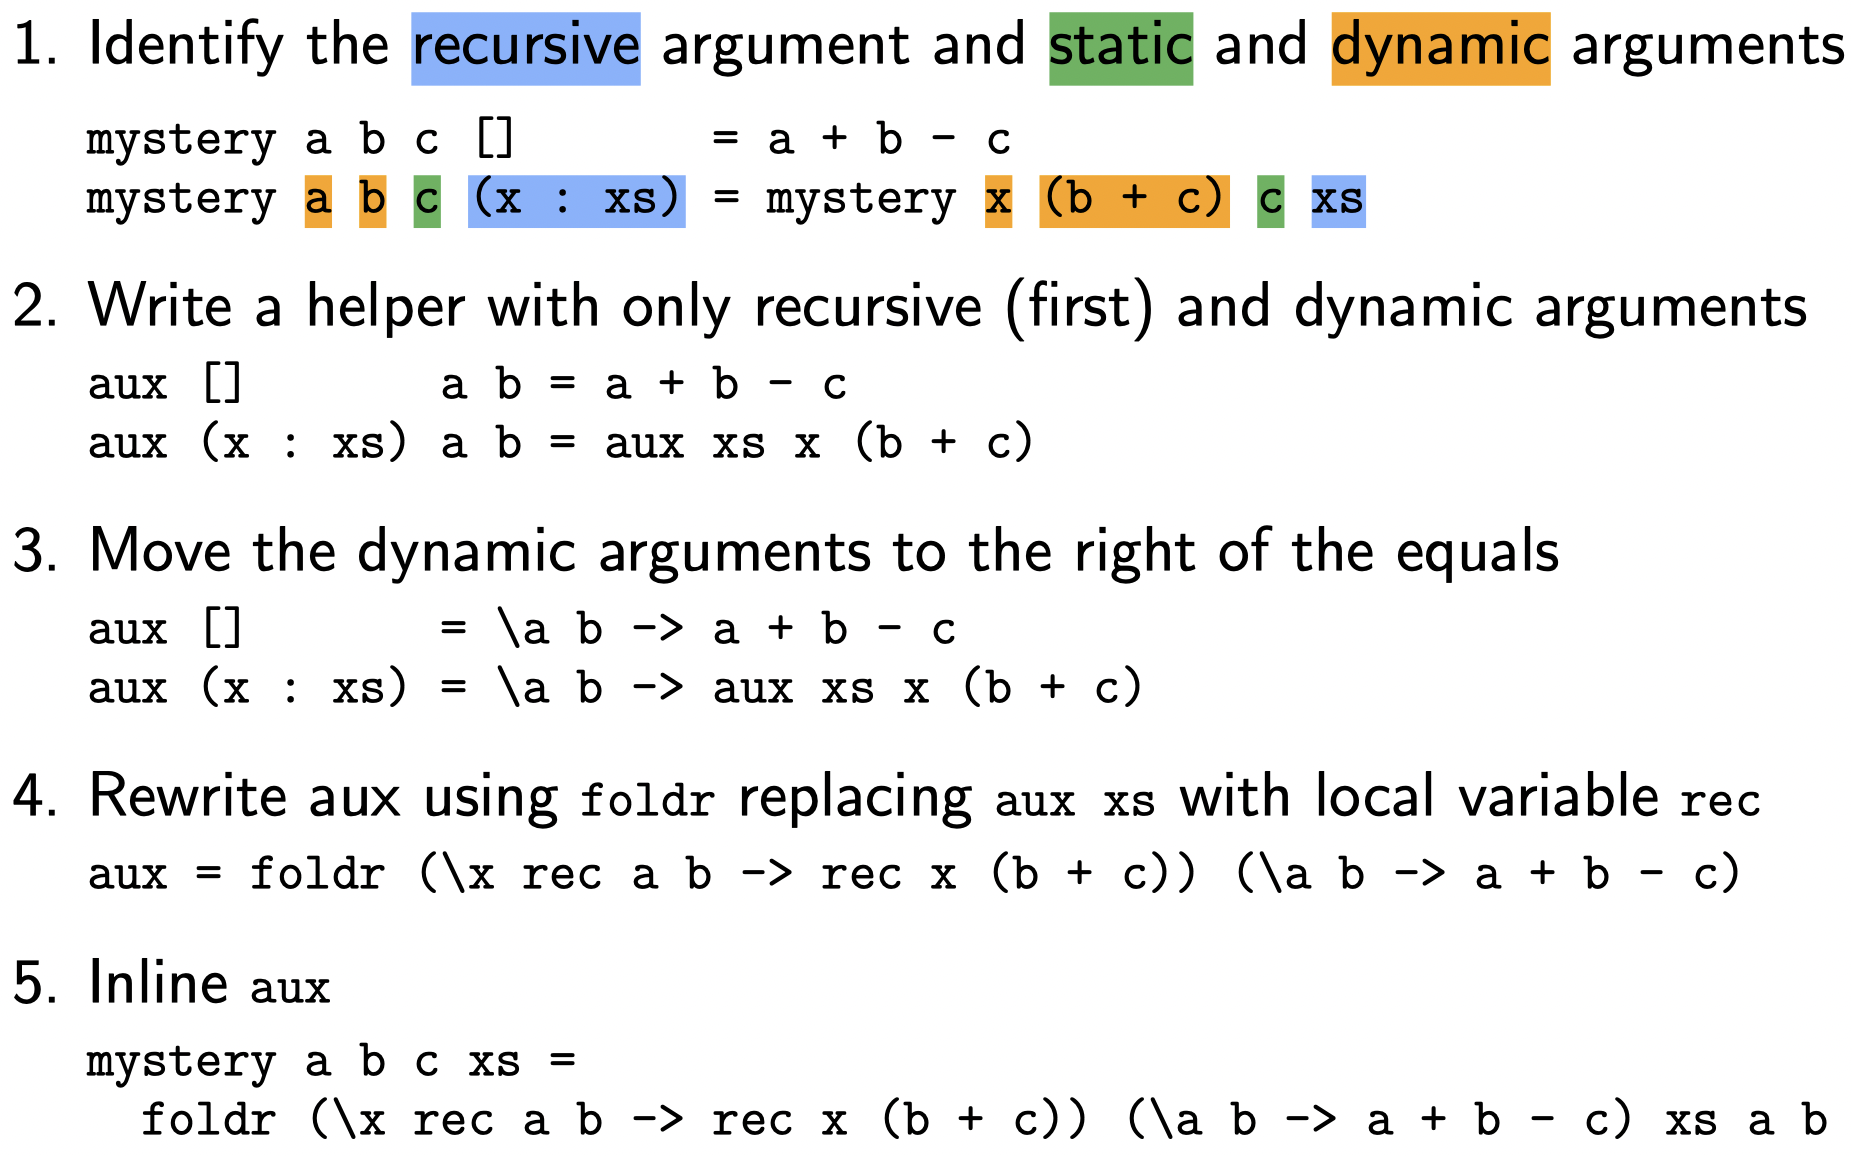
\includegraphics[width=13cm]{../images/FMFP_Fig4-1}
    \centering
\end{figure}

\end{document}